Trabaje para $t\ge0$ con la transformada unilateral de Laplace y entradas causales. Use $H(t-a)=0$ para $t<a$ y $H(t-a)=1$ para $t\ge a$; los valores aislados en saltos no alteran la transformada. Sea $f$ el triángulo de vértices $(0,0),(1,1),(2,0)$, nulo después de $2$, con transformada conocida $F(s)=(1-e^{-s})^2/s^2$. Las gráficas definen $g$ y $h$: $g$ es cero después del último triángulo; $h$ repite indefinidamente el patrón de longitud $6$.
\begin{center}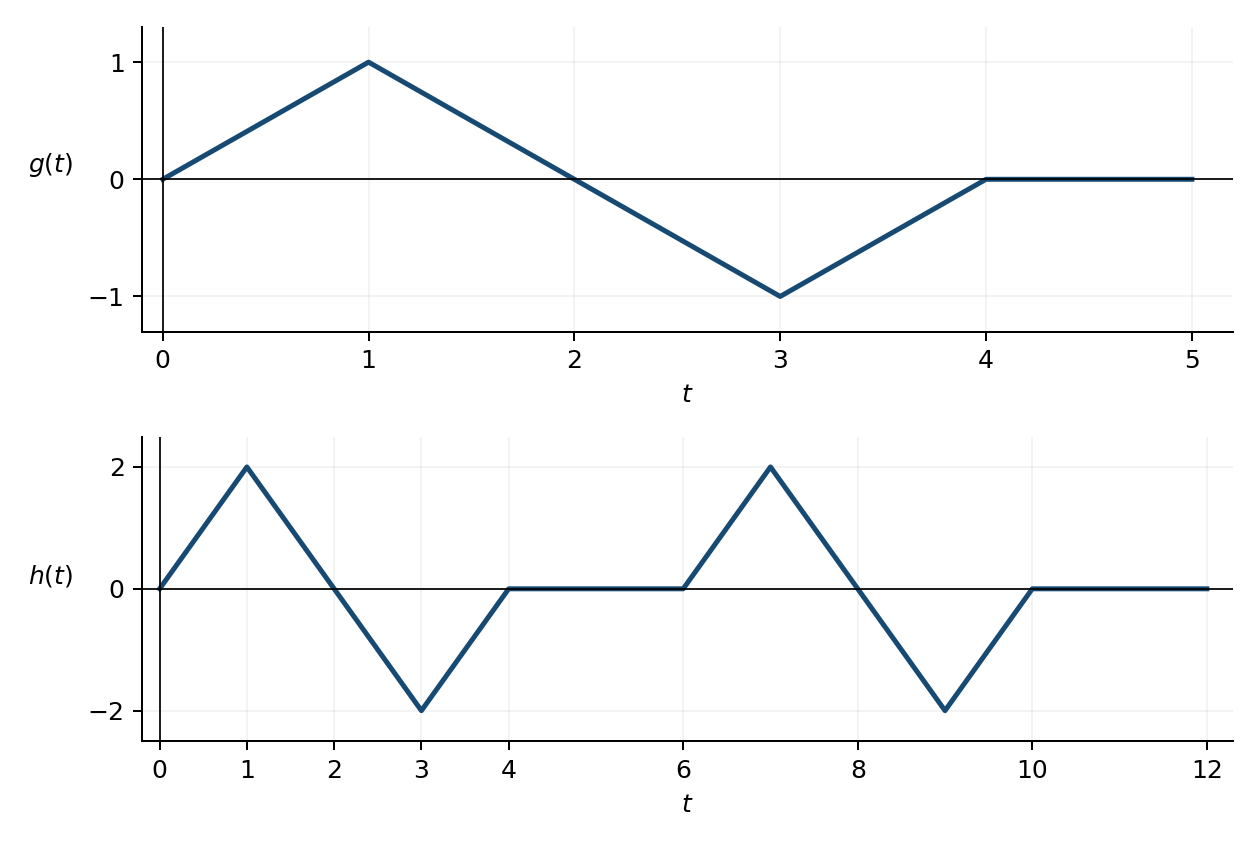
\includegraphics[width=.95\linewidth]{assets/M2-E0230-inputs.png}\end{center}

\begin{enumerate}[label=(\alph*),ref=\alph*,leftmargin=*]
\item Obtenga la transformada de $g$ utilizando $F$.
\item Calcule la transformada de $h$.
\item Resuelva $y''+y=g(t)$, $y(0)=y'(0)=0$.
\end{enumerate}
